\section{Synchronization and protection}

\subsection{Sub topics}

\begin{itemize}
	\item Data integrity - Concurrency challenge.
	\item Mutex and Semaphore.
	\item Mutex and Conditionals.
	\item Producer / Consumer problem.
	\item Dining philosophers.
	\item Dead locks.
\end{itemize}

\subsection{Curriculum}

\begin{itemize}
	\item Slides: "Thread Synchronization I and II".
	\item Kerrisk: Chapter 30: Thread Synchronization.
	\item Kerrisk: Chapter 31: Thread Safety and Per-Thread Storage (Speed read)".
	\item Kerrisk: Chapter 32: Thread Safety and Per-Thread Storage (Speed read)".
	\item Kerrisk: Chapter 53: Posix Semaphores (Named not in focus for this exercise)".
	\item OLA: "Pthread-Tutorial" - chapters 4-6.
	\item OLA: "Producer/Consumer problem".
	\item OLA: "Dining Philosophers problem".
\end{itemize}

\subsection{Exercises}

\begin{itemize}
	\item Posix Threads
	\item Thread Synchronization I \& II
\end{itemize}

\newpage

\subsection{Data integrity - Concurrency challenge}

Selvom informations deling tråde imellem er en af de væsentligste fordele ved multitrådede applikationer, er det vigtigt at se sig for når flere tråde behandler den samme data.
Man bruger termet \textit{critical section} til at referere til et stykke kode der benytter en delt ressource, hvor dette bør gøres \textit{atomic}. Vi har derfor brug for en måde at sikre os eksklusiv adgang når der arbejdes på delte data.

\subsection{Mutex and Semaphore}

En ovenfornævnt kritisk sektion kan defineres ved hjælp af mutexes og semaphorer.

\subsubsection{Mutexes}

En tråd kan tage ejerskab over en mutex, dvs at mutexen låses, og ikke kan tages af andre tråde før den frigives af ejertråden og derved låses op. \\

En mutex skal initialiseres og destrueres.

\begin{itemize}
	\item textit{lock(mut)} - tråden forsøger at tage mutexen. Funktionen er blokerende hvis mutexen er taget.
	\item \textit{trylock(mut)} - samme som \textit{lock()}, men i stedet for at blokere, returneres EBUSY
	\item \textit{timedlock(mut, timeOut)} - samme som \textit{lock()}, hvor der dog her gives et timeout med som parameter, dvs. en tidsbegrænsing for hvor længe tråden skal vente på at få mutexen.
	\item \textit{unlock(mut)} - tråden låser mutexen op. 
\end{itemize}

\subsubsection{Semaphorer}
En semaphor kan beskrives som en counter der tæller hvor meget af en ressource der tilgængelig.
En mutex er det samme som en semaphor der er begrænset til værdierne 0 og 1 (binær).
To typer semaphorer:

\begin{enumerate}
	\item Counted semaphore
	\item Binær semaphore
\end{enumerate}

En semaphor kan ved at inkrementere/dekrementere en counter, holde styr på og begrænse antallet af klienter der opererer på en ressource. En semaphor kan deles på tværs af processer. I en semaphor er der ikke ejerskab, hvilket medfører at en semaphor kan frigives af en client selvom denne ikke taget den.

\paragraph{Named og unnamed semaphorer}
En named semaphor kan benyttes på tværs af urelaterede processer ved brug af dens navn.\todo{Se kommentar i latex koden}
%Er det ikke noget med sem_open(\"name" som parameter?? hvad så når den er unnamed?

En unnamed semaphor bruges som udgangspunkt kun inden for samme process med mindre den er gemt i delt hukommelse. 

Om en semaphor er named eller unnamed defineres i semaphorens initiering.

unnamed: 

\subsection{Mutex and Conditionals}

\subsection{Producer/Consumer problem}
Også kaldet \textit{bounded-buffer problem}.\\

Når vi har to tråde som skal tilgå en data buffer.

\begin{itemize}
	\item En \textbf{Producer} som skal putte data i bufferen.
	\item En \textbf{Consumer} som skal tage data ud af bufferen.
\end{itemize}

Problemet opstår når Produceren forsøger at pushe til en fuld buffer, eller når consumeren forsøger at poppe fra en tom buffer.

Hvis vi lader begge tråde checke om bufferen er tøm/fuld før de gør noget, spilder vi kostbar CPU tid.

\subsubsection{Løsning med Mutex}

\begin{lstlisting}[otherkeywords={item, buffer, unlock, lock, signal}]
// Producers adds item to buffer
void Producer::put(item i)
{
	lock(mtx);
	
	while(size == max_size)
		wait(mtx, producer_cond);
		
	buffer.push(i);
	size++;
	
	unlock(mtx);
	signal(consumer_cond);
}
\end{lstlisting}

\begin{lstlisting}
// Consumers get function
item Comsumer::get()
{
	lock(mtx);
	
	while(size == 0)
		wait(mtx, consumer_cond);
		
	get_from_buffer();
	size--;
	
	unlock(mtx);
	signal(producer_cond);
}
\end{lstlisting}

\subsubsection{Løsning med Semaphore}
\begin{lstlisting}[otherkeywords={}]
empthySlotsSem = create_semaphore(buffer_size)
\end{lstlisting}

\subsection{Dining philosophers}
Wikipedia om problemet findes \href{https://en.wikipedia.org/wiki/Dining_philosophers_problem}{her}.

\begin{figure}[h]
	\centering
	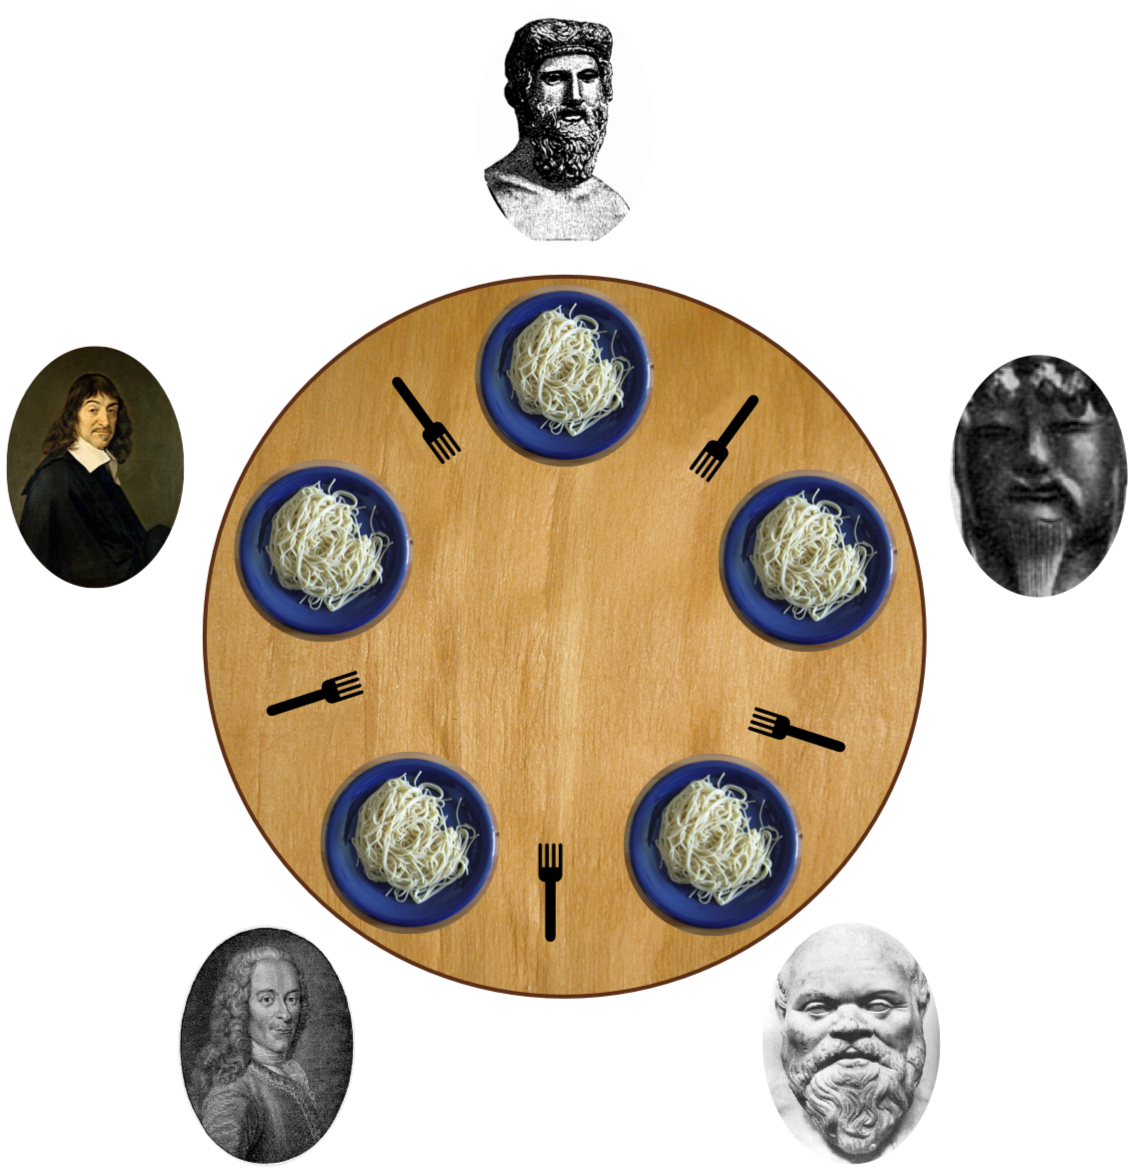
\includegraphics[width=0.5\linewidth]{figs/spm2/dining}
	\caption{Dining philophers problem illustrated. Med uret fra toppen: Platon, Konfuzius, Socrates, Voltaire og Descartes.}
	\label{fig:dining}
\end{figure}

\subsubsection{Løsninger}
I section~\ref{sec:deadlock} er fire betingelser for deadlocks beskrevet. Vores opgave er at bryde mindst én af disse.

\begin{enumerate}
	\item \textbf{Mutual exclution} - Nope, de skal have hver deres egen gaffel.
	\item \textbf{Hold and Wait} eller \textbf{Resource holding} - Heller ikke, de skal have to gafler for at spise.
	\item \textbf{No preemption\footnote{Læs om preemption i section~\ref{sec:execpu}}} - Nix, de må ikke tage hinandens gafler.
	\item \textbf{Circular wait} - Bingo! Vi kan bryde denne cykel!
\end{enumerate}

Dette kan imidlertid gøres på flere måder:

\paragraph{Ressource hierarchy solution}
Dette var Dijkstra's originale løsning på probelmet.

Ved at etablere en bestemt rækkefølge som ressourcerne skal ''tages'' i, kan vi bryde cyklen. For vores tilfælde vil gaflerne blive nummereret. Når en filosof så vil spise skal han først tage gaflen med de \textbf{mindste} nummer.

\paragraph{Arbitrator solution}
Hvis de kun kan samle \textit{begge} eller \textit{ingen} af gaflerne kan samles op kan problemet løses. Dette gøres ved at filosofferne skal spørge en tjener\footnote{Tjeneren kan implementeres som en mutex.} om tilladelse før de tage gaflerne, hvorefter de samler gafler op, indtil de har begge. 

Problemet bliver imidlertid så at kun én filosof kan spise af gangen, selv hvis der er flere gafler ledige.

\paragraph{Chandry/Misra solution}
I 1984 kom K. Mani Chandy og J. Misra med en anden løsning, som tillod at et arbitrært antal ''agents'' kan bruge et arbitrært antal ressourcer.

Den kræver ikke nogen central enhed, men den kræver tilgengæld at enhederne kommunikerer. Se \href{https://en.wikipedia.org/wiki/Dining_philosophers_problem#Chandy.2FMisra_solution}{wiki} for præcis beskrivelse.

\subsection{Dead locks}\label{sec:deadlock}
Deadlock er en situation hvor tråde ikke frigiver deres ressourcer fordi de venter på ressourcer som andre tråde ligeledes holder mens de venter på samme ting.\\

På wikipedia om \href{https://en.wikipedia.org/wiki/Deadlock}{deadlock} kan man læse om de fire betingelser som skal være overholdt for at en deadlock kan opstå:
\begin{enumerate}
	\item \textbf{Mutual exclution}\\
	Mindst én ressource skal være ''holdt'' i et \textit{non-shareable mode}\footnote{Kun én tråd kan bruge ressourcen af gangen.}.
	\item \textbf{Hold and Wait} eller \textbf{Resource holding}\\
	En tråd ''holder'' mindst én ressource og anmoder om flere ressourcer, hvor disse ''holdes'' af andre tråde.
	\item \textbf{No preemption\footnote{Læs om preemption i section~\ref{sec:execpu}}}\\
	En ressource kan kun frigives af tråden som holder den.
	\item \textbf{Circular wait}\\
	En tråd/process venter på en ressource som på tidspunktet holdes af en anden tråd/process. Denne anden tråd venter ligeledes på at den første tråd frigiver sin ressource.
\end{enumerate}

For at deadlocks ikke skal opstå, skal mindst én af de ovenstående betingelser brydes.
